\documentclass[12pt, a4paper]{article}
\usepackage{../../../../../style}
\begin{document}
	\lhead{Группа 91} \chead{Модуль 6 Занятие №2} \rhead{Школа <<Симметрия>>}
	\begin{wrapfigure}{r}{0.4\textwidth}
		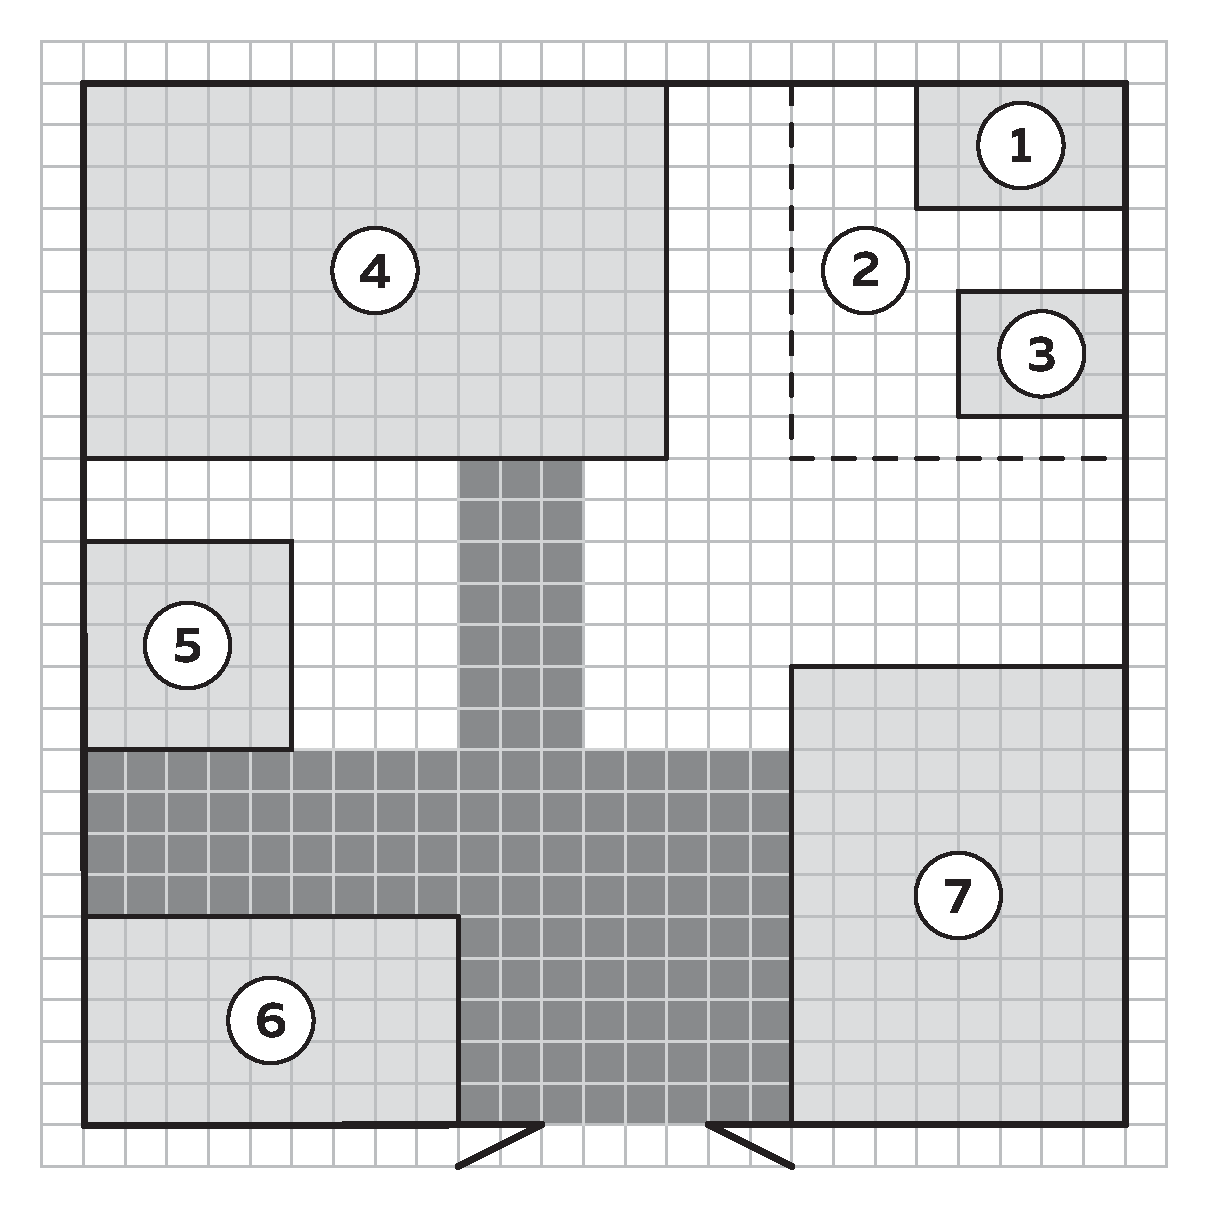
\includegraphics[align=t, width=0.4\textwidth]{plan}
	\end{wrapfigure}
	На плане изображена схема квартиры (сторона каждой клетки на схеме равна 1 м). Вход и выход осуществляются через единственную дверь.
	
	При входе в квартиру расположена прихожая, отмеченная цифрой 6. Из прихожей можно попасть в гостиную, расположенную справа от неё. В квартире есть балкон, занимающий наименьшую площадь. Перед входом в прихожую располагается спальня, а справа от неё — детская комната, в которую можно попасть только из спальни. Рядом со спальней расположен совмещенный санузел площадью 12 м$^2$. Кроме того, в квартире есть кухня.
	
	Пол в гостиной планируется покрыть паркетной доской длиной 1 м и шириной 0,25 м. В квартире проведены газопровод и электричество.
	
	\begin{enumerate}
		\item Для объектов, указанных в таблице, определите, какими цифрами они обозначены на схеме. Заполните таблицу, в ответ запишите последовательность четырёх цифр.
		\begin{center}
			\includegraphics[align=t, width=0.5\textwidth]{table}
		\end{center}
		\item Паркетная доска продаётся в упаковках по 16 шт. Сколько упаковок с паркетной доской требуется купить, чтобы покрыть пол в гостиной?
		\item Найдите площадь, которую занимают спальная комната и детская. Ответ дайте в квадратных метрах.
		\item Насколько квадратных метров площадь гостиной больше площади балкона?
		\item Найдите расстояние $d$ между противоположными углами кухни в метрах. В ответ запишите в виде $\dfrac{d}{\sqrt{2}}$
		\item Хозяин квартиры планирует установить в квартире плиту для готовки. Он рассматривает два варианта:
		газовая плита или электроплитка. Цены на плиты, данные о потреблении и тарифах оплаты даны в таблице.
		\begin{center}
			\includegraphics[align=t, width=0.5\textwidth]{table2}
		\end{center}
		Обдумав оба варианта, хозяин решил установить газовую плиту. Через сколько часов непрерывного
		использования экономия от использования газовой плиты вместо электрической компенсирует разность в
		стоимости установки газовой плиты и электроплитки?
		\newpage
		\item Вычислите:
		\begin{multicols}{2}
			\begin{enumerate}[label=\asbuk*)]
				\item $354\cdot 49:1239+357\cdot48:56$
				\item $\dfrac{6^3\cdot5^2}{3^3\cdot2^4}$
				\item $\left(3\dfrac{1}{3}\right)^3\cdot(0,1)^3:3$
				\item $\sqrt{\dfrac{1}{625}}+2\sqrt{0,64}$
			\end{enumerate}
		\end{multicols}
		\item На координатной прямой отмечена точка А, которая соответствует одному из чисел, указанных ниже. Какому числу она соответствует?
		\begin{center}
			\includegraphics[align=t, width=0.8\textwidth]{ex7}
		\end{center}
		\begin{multicols}{4}
			\begin{enumerate}[label=\arabic*)]
				\item $\dfrac{2}{7}$
				\item $\dfrac{4}{7}$
				\item $\dfrac{10}{7}$
				\item $\dfrac{11}{7}$
			\end{enumerate}
		\end{multicols}
		\item Найдите значение выражения $\dfrac{\sqrt{300}\cdot\sqrt{54}}{\sqrt{5}}$\\
		\textit{В ответе укажите номер правильного варианта.}
		\begin{multicols}{4}
			\begin{enumerate}[label=\arabic*)]
				\item $90\sqrt{2}$
				\item $36\sqrt{5}$
				\item $18\sqrt{10}$
				\item $18\sqrt{30}$
			\end{enumerate}
		\end{multicols}
		\item Решите уравнения:
		\begin{multicols}{2}
			\begin{enumerate}[label=\arabic*)]
				\item $0,5x-3=0,8-1,4x$
				\item $x+0,2=0,4x+3,2$
				\item $\dfrac{2}{3}-3x=\dfrac{1}{2}x-2+x$
				\item $3-\dfrac{x}{5}=\dfrac{x}{7}$
				\item $5-\dfrac{1}{3}x-\dfrac{1}{2}=\dfrac{1}{4}x$
			\end{enumerate}
		\end{multicols}
		\item На тарелке лежат пирожки, одинаковые на вид: 6 с мясом, 9 с капустой и 5 с вишней. Петя наугад
		выбирает один пирожок. Найдите вероятность того, что пирожок окажется с вишней.
		\item Зная длину своего шага, человек может приближённо подсчитать пройденное им расстояние s по
		формуле $s=nl$, где $n$ --- число шагов, $l$ --- длина шага. Какое расстояние прошёл человек, если $l=70$ см, $n=1400$? Ответ выразите в километрах.
		\item Решите неравенство $-3-x>4x+7$.\\ \textit{В ответе укажите номер правильного варианта.}
		\begin{multicols}{2}
			\begin{enumerate}[label=\arabic*)]
				\item $(-\infty;-0,8)$
				\item $(-2;+\infty)$
				\item $(-0,8;+\infty)$
				\item $(-\infty;-2)$
			\end{enumerate}
		\end{multicols}
		\item Решите квадратные уравнения:
		\begin{multicols}{2}
			\begin{enumerate}[label=\asbuk*)]
			\item $5x^2-6x+1,75=0$
			\item $\dfrac{5}{4}x^2-x+\dfrac{1}{9}=0$
			\item $(2x+3)^2-(x-2)^2=5$
			\end{enumerate}
		\end{multicols}
	\end{enumerate}
\end{document}